\documentclass[t]{beamer}
\usetheme{Warsaw}
\usecolortheme{seahorse}
\usepackage{array}
%\usepackage{graphicx}
\usepackage{amssymb,amsmath,mathrsfs,amsfonts}
%\usepackage[colorhighlight,display]{texpower}
%\usepackage{caption}
%\usepackage[all]{xy}
\usepackage{beamerthemesplit}
\mode<presentation>
%\usepackage{pause}
\usepackage{ulem}  % for strikethroughs
\usepackage{cancel} % for strikethroughs in math mode 
\usepackage{tikz}
\usetikzlibrary{shapes}
\usepackage{hyperref}
\hypersetup{pdfpagemode=FullScreen}
\usepackage{ifthen}
\usepackage{animate}
\usepackage{color}
\usepackage{type1cm}  % used for watermarking
\usepackage{eso-pic}  % used for watermarking


\theoremstyle{plain}
\newtheorem{prop}{Proposition}
\newtheorem{thm}[prop]{Theorem}
\newtheorem{lem}[prop]{Lemma}
\newtheorem{cor}[prop]{Corollary}
\theoremstyle{definition}
\newtheorem{dfn}{Definition}
\newtheorem{rem}[prop]{Remark}
\newtheorem{ex}{Example}[section]
%\newtheorem{note}{Note}[section]
\newtheorem{exercise}{Exercise}[section]
\newcommand{\nin}{\noindent}
\newcommand{\ds}{\displaystyle}
\renewcommand{\figurename}{Figure \arabic{figure}}



\renewcommand*\familydefault{\sfdefault} 




%%%%%%%%%%%%%%%%%%%%%%%%%%5
%%%%%%%%%%%%%%%%%%%%%%%%%%%%
%%%% some commands that have different meaning in the article/presentation modes

\newcommand{\vvfill}{\mode<presentation>{\vfill}  \mode<article>{\medskip}}   %vfill in presentation only
\newcommand{\sketchspace}{ 
\mode<article>{ \medskip\noindent{\textbf{Sketch:}} \vspace*{6cm} }
\mode<presentation>{ } 
}
\newcommand{\examplespace}{ 
\mode<article>{ \medskip\noindent{\textbf{Example:}} \vspace{6cm} }
\mode<presentation>{ } 
}
\newcommand{\artsmspace}{\mode<article>{\vspace*{2cm}} }  %small space in article mode
\newcommand{\artlargespace}{\mode<article>{\vspace*{6cm}} }  %large space in article mode

\newcommand{\dx}{\,dx}

\newcommand{\soln}{{\textbf{Solution: }}\,\,\,}
\newcommand{\disp}{\displaystyle}

\newcommand{\makedate}{\vvfill
\begin{picture}(10,10)  
\put(260,-20){\mbox{\tiny{\today}}}
\end{picture}
}

\newcommand{\pd}[2]{\dfrac{\partial#1}{\partial#2}}
\newcommand{\pD}[2]{\dfrac{\partial^2#1}{\partial#2^2}}
\newcommand{\pdd}[3]{\dfrac{\partial^2#1}{\partial#2 \partial#3}}


\normalem %stops the ulem package making all the emphs into underlines....
 
 
 
 \newcommand{\refandrev}[2]{
 \begin{small}
  \hspace{6cm}
  \begin{minipage}[r]{8cm}
  Stewart,    Chapter #1   \\
  Review:  \parbox[t]{6cm}{#2}
\end{minipage}
\end{small}
}



\newcounter{heading}
\setcounter{section}{1}
\setcounter{heading}{0}

\newcommand{\makeheading}[1]{\medskip\begin{large}\noindent\textbf{{#1}}\end{large}\smallskip}

%\newenvironment{head}[1]{\medskip\stepcounter{heading}\noindent\textbf{\hspace{0.2cm}{#1}.}}{}
\newcommand{\newhead}[1]{\medskip\stepcounter{heading}\noindent\textbf{\hspace{0.2cm}{#1}.}}


\newcommand{\pf}[1]{\noindent\textit{Proof.}\vspace*{#1 cm}}
\newcommand{\sol}[1]{\noindent\textit{Solution.}\vspace*{#1 cm}}
\newcommand{\further}[1]{\begin{small}\noindent\textit{Further reading: #1}\end{small}}
\newcommand{\exr}[1]{\begin{footnotesize}\noindent\textit{\textbf{Exercises:} Stewart #1}\end{footnotesize}}


% Sets of numbers
\newcommand{\C}{\mathbb{C}}
\newcommand{\RR}{\mathbb{R}}
\newcommand{\Z}{\mathbb{Z}}
\newcommand{\N}{\mathbb{N}}
\newcommand{\Q}{\mathbb{Q}}

% Partitions
\newcommand{\PP}{\mathcal{P}}

% Limits
\newcommand{\limm}[1]{\displaystyle \lim_{x\to #1}}

% Backslash
\newcommand{\bs}{\backslash}

% functions
\newcommand{\cosec}{\mathrm{cosec}}
\newcommand{\cosech}{\mathrm{cosech}}
\newcommand{\sech}{\mathrm{sech}}
\newcommand{\Li}{\mathrm{Li}}
\newcommand{\si}{\mathrm{Si}}
\newcommand{\erf}{\mathrm{erf}}

% Domain and Range
\newcommand{\Dom}{\mathrm{Dom}}
\newcommand{\Codom}{\mathrm{Codom}}
\newcommand{\Range}{\mathrm{Ran}}



\title{Week 3:  Derivatives}
%\date{July 6 -- August 10, 2012}

\begin{document}

\frame{\titlepage}

\setcounter{tocdepth}{2}
\frame{\tableofcontents

}

\AtBeginSection[]
{
\begin{frame}<beamer> 
\tableofcontents[currentsection]  % show TOC and highlight current section
\end{frame}
}


\section{Derivatives}
\subsection{Meaning and Computation of derivatives}

\frame
{
\frametitle{Average rate of change}
\begin{dfn}
\begin{multline*} \text{Average rate of change of }f(x)\text{ between }x=a\text{ and }x=b\\=\frac{f(b)-f(a)}{b-a}\\
\end{multline*} 
\end{dfn}
}

\frame
{
\frametitle{Average rate of change}
\begin{figure}[t]
\begin{center}
\includegraphics[scale=0.4]{image011.jpg}
\end{center}
\end{figure}

Average rate of change of $f(x)$ between $x=-10$ and $x=0$ \\ 
 $=$ Slope of the \textbf{secant line} joining $(-10, 48)$ and $(0,88)$.
 \[ =\frac{f(0)-f(-10)}{(0-(-10))}
=\frac{88-48}{10}=\frac{40}{10}=4. \]
}

\frame
{
\frametitle{Instantaneous rate of change}
\begin{dfn}
{\em Instantaneous rate of change of a function $f(x)$ at $x=a$} is \[\lim_{x\to a}\frac{f(x)-f(a)}{x-a}\]
Taking $x=a+h$, $h\to 0$ as $x\to a$. So, we can rewrite as 
\[\lim_{h\to 0}\frac{f(a+h)-f(a)}{h}\]\\
The second definition is also known as \textbf{derivative}.  Also denoted as $f'(x)$ or $\dfrac{dy}{dx}$ or $\dfrac{df}{dx}$ or $\dfrac{d}{dx}f(x)$.   We can also have \textbf{higher derivative} (e.g., 2) which is denoted as $f''(x)$ or $\dfrac{d^2y}{dx^2}$ or $\dfrac{d}{dx}(\dfrac{dy}{dx})$. 
\end{dfn}

}

\frame
{
\frametitle{Instantaneous rate of change}
Instantaneous rate of change of $f(x)$ at $x=a$ \\= Slope of the \textbf{tangent} line to $f(x)$ at the point $x=a$.

\begin{figure}[h] %  figure placement: here, top, bottom, or page
     \centering
     \includegraphics[width=2.5in]{Tangent_as_Secant_Limit.png}
%     \caption{Secant lines between $P$ and $Q$, as $Q$ approaches $P$}
     \label{fig:4}
  \end{figure}
  }
  
 \frame
{
	\frametitle{Example}
	Find the equation of the tangent line to the graph $f(x)= x^2$ at $(1, 1)$. 
	
	\[\begin{array}{lcl}
\disp{\lim_{h\to 0}} \dfrac{f(1+h)-f(1)}{h} &=& \disp{\lim_{h\to 0}} \dfrac{(1+h)^2- 1^2}{h}\\ 
&=& \disp{\lim_{h\to 0}} \dfrac{2h+h^2}{h}\\ 
&=& \disp{\lim_{h\to 0}}  (2+h) =2 \end{array}\] 

	\vspace{2em}	
	
	Using the point-slope form ($y - y_1 = m(x - x_1)$), we can find the tangent line at $(1, 1)$ as
	$y - 1 = 2(x - 1)$  or $y = 2x - 1$.
}

\frame
{
	\frametitle{Example}
	Find the equation of the tangent line to the graph $f(x)= \dfrac{3}{x}$ at $(3,1)$. 
	
	\[\begin{array}{lcl}
\disp{\lim_{h\to 0}} \dfrac{f(3+h)-f(3)}{h} &=& \disp{\lim_{h\to 0}} \dfrac{\dfrac{3}{3 + h} - 1}{h}\\ 
&=& \disp{\lim_{h\to 0}} -\dfrac{1}{3 + h} = -\dfrac{1}{3}\\ \end{array}\] 

	\vspace{2em}	
	
	Using the point-slope form ($y - y_1 = m(x - x_1)$), we can find the tangent line at $(3, 1)$ as
	$y - 1 = -\dfrac{1}{3}(x-3)$ which becomes $x + 3y - 6 = 0$.
}

\frame
{
	\frametitle{Example}
	Find $f'$ of $f(x)= x^3 - x$. 
	
	\[\begin{array}{lcl}
 \disp{\lim_{h\to 0}} \dfrac{f(x+h) - f(x)}{h}&=& \disp{\lim_{h\to 0}} \dfrac{[(x + h)^3 - (x + h)] - [x^3 - x]}{h}\\ 
&=& \disp{\lim_{h\to 0}} \dfrac{x^3 + 3x^2h + 3xh^2 + h^3 - x - h - x^3 + x}{h}\\ 
&=& \disp{\lim_{h\to 0}} \dfrac{3x^2h + 3xh^2 + h^3 - h}{h}\\ 
&=& \disp{\lim_{h\to 0}} 3x^2 + 3xh + h^2 -1 \\&=& 3x^2 -1\\ 
\end{array}\] 
}

\begin{frame}
\makeheading{Self-Exercise}

\begin{enumerate}

\item Find the derivative of $y = x^2 - 3x$ at $x = 2$ 
\begin{itemize}
	\item Ans: $1$
\end{itemize}

\item Find $f'$ of $\dfrac{1-x}{2+x}$ 
\begin{itemize}
	\item Ans: $-\dfrac{3}{(2+x)^2}$
\end{itemize}

\item Find $f'$ of $\sqrt{x}$  \qquad (Hint: Multiply with $\dfrac{\sqrt{x + h} + \sqrt{x}}{\sqrt{x + h} + \sqrt{x}}$)
\begin{itemize}
	\item Ans: $\dfrac{1}{2\sqrt{x}}$
\end{itemize}

\item Find equation of the tangent line of $y = x^2 - 8x + 9$ at point $(3, -6)$
\begin{itemize}
	\item Ans: $y = -2x$
\end{itemize}

\end{enumerate}

\end{frame}


%\begin{frame}
%\frametitle{Important example}
%
%\noindent Suppose an object moves along a straight line according to the equation of motion $y = f(t)$, where $y$ is the displacement of the object from the origin at time $t$, then we call $f$ the \emph{position function} of the object.  The \emph{velocity} of the object at $t=a$ is defined to be the instantaneous rate of change of the position function when $t=a$.  The \emph{speed} of the object at $t=a$ is defined to be the absolute value of the velocity when $t=a$.\\
%
%\noindent Suppose an arrow is shot upwards on the moon with a velocity of $58$ meters per second, then its height in meters after $t$ seconds is given by
%\[H = 58t - 0.83t^{2}.\]
%Find the velocity and speed of the arrow after $1$ second.
%\end{frame}

\subsection{Differentiable functions}

%\begin{frame}
%\begin{dfn} Suppose that $f$ is defined on some open interval containing the point $x$. We say that $f$ is \textit{differentiable} at $x$ if $f'(x)$ exists.\end{dfn}
%
%\newhead{Remark on notation} Other notation for $f'(x)$  includes $\frac{d}{dx}f(x)$ and $\frac{df}{dx}(x)$ . If $y=f(x)$ then the derivative is often denoted by $y'$ or $\frac{dy}{dx}$. The ratio
%\[\frac{f(x+h)-f(x)}{h}\]
%is called the \textit{difference quotient} for $f$ at the point $x$.
%
%\vspace*{.1cm}
%
%\newhead{Example}
%
%\noindent If $f(x) = |x|$, does $f'(0)$ exist?
%
%\end{frame}

\begin{frame}

\begin{dfn}
A function is differentiable at $x = a$ if $f'(a)$ exists.
\end{dfn}

\begin{thm}
If $f$ is differentiable at $a$ then it is continuous at $a$. 
\end{thm}

\begin{thm}
If $f$ is not continuous at $x = a$ then $f$ is not differentiable at $x=a$. 
\end{thm}

\begin{thm}
If $f$ is continuous at $a$ $f$ may or may not be differentiable at $x=a$. 
\end{thm}
e.g., $f(x) = |x|$ is cont. at $x=0$ but is not differentiable at $x =0$

\end{frame}

\begin{frame}

What are places where this graph is \textbf{NOT differentiable} and why?

	\begin{figure}[l]
	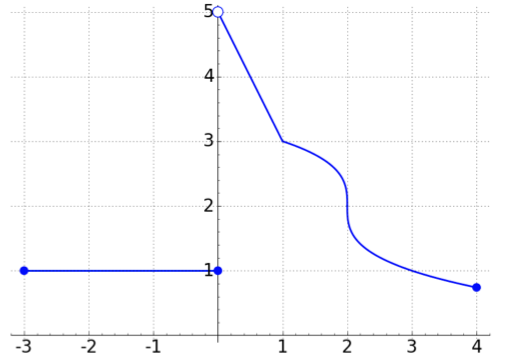
\includegraphics[scale=.25]{fig/differentiable0}
	\label{fig}
	\end{figure}	

\begin{itemize}
	\item -3: left limit DNE thus discontinuous
	\item 0: discontinuous
	\item 1: sharp corner
	\item 2: the slope is $\infty$
	\item 4: right limit DNE thus discontinuous
\end{itemize}

\end{frame}

%\begin{frame}
%\frametitle{Higher order derivatives}
%
%\noindent If $f$ is a differentiable function with derivative $f'$, sometimes $f'$ may also be differentiable. If this is the case, then the derivative of $f'$ is denoted $f''$ and called the \textit{second derivative of $f$}. If $y=f(x)$ then we can also write
%\[f''(x)=\frac{d}{dx}\left(\frac{dy}{dx}\right)=\frac{d^2y}{dx^2}.\]
%If $f''$ is differentiable then its derivative $f'''$ is called the \textit{third\\ derivative of $f$}. The prime notation $f'''$ is only practical until the third derivative. For higher order derivatives we introduce new notation.
%\end{frame}
%
%\begin{frame}
%\frametitle{Higher order derivatives}
%
%
%\newhead{Notation} Suppose that $f$ can be differentiated $n$ times. Then its $n$th derivative is denoted by $f^{(n)}$. If $y=f(x)$ then we also write
%\[f^{(n)}(x)=\frac{d^ny}{dx^n}.\]
%
%\noindent Higher order derivatives have various interpretations depending on the context. A geometric interpretation of the second derivative will be given in the next chapter. One interpretation that features in mechanics is that of \emph{acceleration}. As before, suppose that the position of a object that moves in a straight line is given by $y(t)$ at time $t$.  Then $v(t) = y'(t)$ is the velocity of the particle and $a(t) = v'(t)$ is its acceleration at time $t$.  Note that $a(t) = y''(t)$, so acceleration is the second derivative of position.
%\end{frame}

%\begin{frame}
%\frametitle{Rules for differentiation}
%
%\noindent So far we have calculated derivatives working directly from the definition, that is, by taking the limit as $h \to 0$ of the difference quotient. However, in practice this is often both difficult and tedious.  Luckily, there exist some nice rules that make it quite easy to compute the derivatives of most functions we are familiar with.
%
%\newhead{Some basic derivatives}
%\begin{center}
%\begin{tabular}{|l|l|}
%\hline
%$f(x)$					& $f'(x)$			\\
%\hline
%$C$, where $C$ is a constant		& $0$				\\
%$x^n$, where $n$ is a real number	& $nx^{n-1}$			\\
%$\sin x$				& $\cos x$			\\
%$\cos x$				& $-\sin x$		\\
%$e^x$				& $e^x$ \\
%$\ln x$				& $1/x$\\
%\hline
%\end{tabular}
%\end{center}
%\end{frame}


\section{Rules for differentiation}

\subsection{Sum, Product, Quotient, Exponential, Chain}

\frame
{
\footnotesize
\frametitle{Rules for differentiation}
\label{tues}
\begin{enumerate}
\item \textbf{Constant Rule}  $f(x) = c \Rightarrow   f'(x) = 0.$\\  
\item \textbf{Power Rule}  $f(x) = x^n    \Rightarrow   f'(x) = nx^{(n-1)},$  for any  $n\in \mathbb{R}$.\\  
\item \textbf{Scalar Multiplication Rule} $ (kf(x))' = kf'(x)$ for any $k\in \mathbb{R}$.\\  
\item \textbf{Sum/Difference Rule}  $[u(x)\pm v(x)]' = u'(x) \pm v'(x).$\\  
\item \textbf{Product Rule} $[u(x)v(x)]' = u'(x)v(x) + u(x)v'(x)$.\\  
\item \textbf{Quotient Rule} $\left[\dfrac{u(x)}{v(x)} \right]'= \dfrac{ u'(x)v(x) - u(x)v'(x)}{[v(x)]^2}$, when $v(x)\neq 0$. \\    
\item {\bf Exponential Rule} If $f(x)=e^{ax}$, $f'(x)=ae^{ax}$. \\  
\item {\bf Logarithm Rule} if $f(x)=\ln x$, $f'(x)=\frac{1}{x}$, for $x\neq 0$. 
\item \textbf{Chain Rule} If $h(x)=f\circ g(x)$ is the composition of two functions $f$ and $g$, then 
\[
h'(x) = f'[g(x)]\cdot g'(x).
\]
\item \textbf{Trigonometric Rule} 
\begin{itemize}
	\item $\sin{x} \Rightarrow \cos{x}$; $\cos{x} \Rightarrow-\sin{x}$; $\tan{x} \Rightarrow \sec^2{x}$
	\item $\cot{x} \Rightarrow -\csc^2{x}$; $\sec{x} \Rightarrow \sec{x}\tan{x}$; $\csc{x} \Rightarrow -\csc{x}\cot{x}$
\end{itemize}

\end{enumerate}
}

\frame
{
	\frametitle{Example}
	Find derivative of $f(x)=\sqrt{x} + \sqrt{\pi}$. 
	
	\begin{align*}
  	&= \dfrac{d}{dx}\sqrt{x} + \dfrac{d}{dx}\sqrt{\pi} \\
  	&= \dfrac{d}{dx}x^{\frac{1}{2}} + \dfrac{d}{dx}\sqrt{\pi} \\
  	&= \dfrac{1}{2}x^{\frac{1}{2}-1} + 0\\
  	&= \dfrac{1}{2}x^{-\frac{1}{2}}  = \dfrac{1}{2\sqrt{x}}\\
	\end{align*}	
}

\frame
{
	\frametitle{Example}
	Find derivative of $\pi t \sqrt{t}e^t$. 
	
	\begin{align*}
  	&=\pi \dfrac{d}{dt} ( t^\frac{3}{2}e^t ) \\
  	&=\pi(e^t * \dfrac{d}{dt}t^\frac{3}{2} + t^\frac{3}{2} * \dfrac{d}{dt}e^t)\\
  	&=\pi(e^t * \frac{3}{2} * t^\frac{1}{2} + t^\frac{3}{2} * e^t)\\
	\end{align*}	
}

\frame
{
	\frametitle{Example}
	Find derivative of $g(x) = ex^2 + 2e^x + xe^2 + x^{e^2}$. 
	
	\begin{align*}
  	&=e* \dfrac{d}{dx}(x^2) + 2* \dfrac{d}{dx}(e^x) + e^2* \dfrac{d}{dx}(x) + \dfrac{d}{dx}(x^{e^2}) \\
  	&= 2ex + 2e^x + e^2(1) + e^2x^{e^2-1}\\
	\end{align*}	
}

\frame
{
	\frametitle{Example}
	Find derivative of $\dfrac{z^2}{z^3 + 1}$. 
	
	\begin{align*}
  	&=\dfrac{(z^3 + 1)*2z - z^2(3z^2 + 0)}{(z^3 + 1)^2} \\
  	&=\dfrac{2z^4 + 2z - 3z^4}{(z^3 + 1)^2} \\
  	&=\dfrac{2z - z^4}{(z^3 + 1)^2} \\
	\end{align*}	
}

\frame
{
	\frametitle{Example}
	Find derivative of $\sqrt{sin{x}}$. 
	
	\vspace{3em}

	We can use the chain rule.  Let $g(x) = \sin{x}$ and $f(u) = u^{\frac{1}{2}}$	
		
	\begin{align*}
  	f' &= f'(g(x)) * g'(x)\\
  	&= \dfrac{1}{2}(\sin{x})^{-\frac{1}{2}} * \cos{x}\\
	\end{align*}	
	
}

\frame
{
	\frametitle{Example}
	Find derivative of $e^{\sin{x^2}}$.    (Hint: 3 chains)
	
	\vspace{3em}

	Let $g(x) = e^{x}$ and $f(u) =  \sin{u}$ and $h(t) = t^2$
	
	\begin{align*}
  	&= e^{\sin{x^2}} * \dfrac{d}{dx} \sin{x^2}\\
  	&= e^{\sin{x^2}} * \cos{x^2} * \dfrac{d}{dx} x^2\\
  	&= e^{\sin{x^2}} * \cos{x^2} * 2x\\
	\end{align*}	
	
}

\frame
{
	\frametitle{Example}
	Find derivative of $5^x$. 
	
	\vspace{3em}

	Since $5 = e^{\ln{5}}$, thus $5^x = 	(e^{\ln{5}})^x$
	
	\begin{align*}
  	&= \dfrac{d}{dx} e^{\ln{5} x}\\
  	&= e^{\ln{5}x} * \ln{5}\\
  	&= 5^x * \ln{5}\\ 
	\end{align*}	
	
	Note: $\dfrac{d}{dx} a^x = a^x \ln{a}$
	
}

\begin{frame}
\makeheading{Self-Exercise}

\begin{enumerate}

\item Find the derivative of $g(t) = 4t^2 + \dfrac{1}{4t^2}$ 
\begin{itemize}
	\item Ans: $8t - \dfrac{1}{2t^3}$
\end{itemize}

\item Find the derivative of $y = e^3$ 
\begin{itemize}
	\item Ans: $0$
\end{itemize}

\item Find $f''$ of $(t^2 -1)*e^t$ 
\begin{itemize}
	\item Ans: $e^t(t^2 + 4t+1)$
\end{itemize}

\item Find derivative of $\dfrac{xe^x}{x^2 + \pi e^x}$ 
\begin{itemize}
	\item Ans: $\dfrac{x^2 + \pi e^x(xe^x + e^x) - xe^x(2x + \pi e^x)}{(\pi e^x + x^2)^2}$
\end{itemize}

\item Find derivative of $5(\tan{x} + \sec{x})^3$ 
\begin{itemize}
	\item Ans: $15(\tan{x} + \sec{x})^2 * \sec^2{x} + \sec{x}\tan{x}$
\end{itemize}

\end{enumerate}

\end{frame}

\subsection{Inverse Trigonometric Functions}

\frame
{
\frametitle{Derivatives of inverse trig functions}

\footnotesize

Note: $y = \sin^{-1}{x}$  means $\sin y = x$.  Another notation is $y=\arcsin{x}$
\begin{enumerate}
\item $\dfrac{d}{dx}\sin^{-1}{x} = \dfrac{1}{\sqrt{1-x^2}}$
\item $\dfrac{d}{dx}\cos^{-1}{x} = -\dfrac{1}{\sqrt{1-x^2}}$
\item $\dfrac{d}{dx}\tan^{-1}{x} = \dfrac{1}{1+x^2}$
\item $\dfrac{d}{dx}\cot^{-1}{x} = -\dfrac{1}{1+x^2}$
\item $\dfrac{d}{dx}\sec^{-1}{x} = \dfrac{1}{x(\sqrt{x^2 - 1})}$
\item $\dfrac{d}{dx}\csc^{-1}{x} = -\dfrac{1}{x(\sqrt{x^2 - 1})}$
\end{enumerate}
}

\frame
{
	\frametitle{Example}
	Find derivative of $y = \tan^{-1}\big(\dfrac{a + x}{a - x}\big)$ 
	
	\vspace{0.5em}
	
	\begin{align*}
  	\dfrac{dy}{dx}&= \dfrac{1}{1 + (\dfrac{a+x}{a-x})^2} * \dfrac{d}{dx} (\dfrac{a + x}{a - x})\\
  	\dfrac{dy}{dx}&= \dfrac{1}{1 + (\dfrac{a+x}{a-x})^2} * \dfrac{(a-x)*1 - (a+x)(-1)}{(a-x)^2}\\
  	\dfrac{dy}{dx}&= \dfrac{a - x + a + x}{(1 + \dfrac{(a + x)^2}{(a - x)^2})(a-x)^2}\\
  	\dfrac{dy}{dx}&= \dfrac{a}{a^2 + x^2}\\
	\end{align*}	
	
}

%
%\begin{frame}
%\frametitle{Sum, difference, and constant multiple rules}
%
%\newhead{True or false?}
%\begin{enumerate}
%\item[(i)] If $f(x) = \sin(x)$ and $g(x) = e^{x}$, then $(f+g)'(x) = \cos(x) + e^{x}$.
%
%%\vspace*{2cm}
%\item[(ii)] If $f(x) = x^{2},$ $g(x) = x^{-3}$, and $h(x) = x^{4}$, then\\ $(f+g+h)'(x) = 3x^{3}$.
%
%%\vspace*{2 cm}
%\item[(iii)] If $C = \pi$, then $\frac{d}{dx}(C^{2}) = 2\pi$.
%%\vspace*{2 cm}
%\end{enumerate}
%\end{frame}
%
%\begin{frame}
%\frametitle{The product and quotient rules}
%
%\noindent If $f$ and $g$ are both differentiable, then 
%\begin{enumerate}
%\item[(i)] $(fg)' = fg' + gf'$ \qquad (the \emph{product rule})
%\item[(ii)]$(\frac{f}{g})' =  \frac{gf' - fg'}{g^{2}}$ \qquad (the \emph{quotient rule}).
%\end{enumerate}
%\noindent That is, $fg$ is differentiable with derivative given by formula (i), and if $\frac{f}{g}$ is defined, then it is differentiable, with derivative given by formula (ii). \emph{Note that these formulas are not particularly intuitive!
%
%\vspace*{.5 mm}
%\newhead{Examples}} 
%\begin{enumerate}
%\item[(i)] Compute the derivative of $y = x^{2}\sin x$
%\vspace*{1mm}
%\item[(ii)] Compute the derivative of $F(x) = \dfrac{3x^{2} + 2\sqrt{x}}{x}.$
%\end{enumerate}
%\end{frame}
%
%\begin{frame}
%\frametitle{The chain rule}
%
%\begin{thm} Suppose that $g$ is differentiable at the point $x$ and $f$ is differentiable at the point $g(x)$. Then $f\circ g$ is differentiable at $x$ and
%\[(f\circ g)'(x)=f'(g(x))g'(x).\]
%\end{thm}
%
%\smallskip
%
%\noindent\textit{Remark:} Sometimes the chain rule is written as
%\[\frac{dy}{dx}=\frac{dy}{du}\cdot\frac{du}{dx}.\]
%While this is easier to remember, it omits some important information, namely the fact that $f'$ is evaluated at $g(x)$.
%
%
%\newhead{Example} Suppose that $y=\sin(x^3+2x)$. Find $\dfrac{dy}{dx}$.
%\end{frame}
%
%\begin{frame}
%\newhead{Examples}
%\begin{enumerate}
%\item[(i)] Differentiate $y = (x^{3} - 1)^{100}$.
%
%\item[(ii)] Differentiate the function $g(t) = \big( \frac{t-2}{2t + 1}\big)^{9}$.
%
%\item[(iii)] If $f(x) = \sin(\cos(\tan x))$, what is $f'(x)$?
%
%\item[(iv)] Here is a table of values for $f, g, f', g'.$
%
%\begin{center}
%\begin{tabular}{ l l l l l}
%    \hline
%    $x$ & $f(x)$ & $g(x)$ & $f'(x)$ & $g'(x)$ \\ \hline
%    1 & 3 & 2 & 4 & 6\\ 
%    2 & 1 & 8 & 5 & 7\\ 
%    3 & 7 & 2 & 7& 9 \\
%    \hline
%    \end{tabular}\end{center}
%\noindent 
%\begin{enumerate}
%\item[(a)] If $h(x) = f(g(x))$, find $h'(1)$.
%\item[(b)] If $H(x) = g(f(x))$, find $H'(1)$.
%\end{enumerate}
%\end{enumerate}
%\end{frame}
%
%
%
%\begin{frame}
%\noindent The following example cannot be solved using the rules for differentiation (why not?). We must work directly from the difference quotient.
%
%\newhead{Example} Suppose that $f$ with domain $\RR$ is defined by
%\[
%f(x)=
%\begin{cases}
%x\sin\frac{1}{x}&\mbox{if }x\neq0\\
%0&\mbox{if }x=0.
%\end{cases}
%\]
%Determine whether or not $f$ is differentiable at $0$.
%\vfill
%
%\newhead{Exercise} Is $
%f(x)=
%\begin{cases}
%x^2\sin\frac{1}{x}&\mbox{if }x\neq0\\
%0&\mbox{if }x=0
%\end{cases}
%$\\
%differentiable at $0$? 
%\end{frame}

\section{Implicit differentiation}

\begin{frame}
\frametitle{Implicit differentiation}

	Find derivative of $9x^2 + 4y^2 = 25$ at point $(1, 2)$
		
	\begin{align*}
  	\dfrac{d}{dx}(9x^2 + 4y^2) &= \dfrac{d}{dx}(25)\\
  	9 \dfrac{d}{dx}x^2 + 4 \dfrac{d}{dx} y^2 &= 0\\
  	9 * 2x + 4 * 2y \dfrac{dy}{dx} &= 0\\
  	\dfrac{dy}{dx} &= \dfrac{-9}{4} * \dfrac{x}{y}\\
	\end{align*}	

	\vspace{-2em}	
	
	At point $(1, 2)$,  $\dfrac{dy}{dx} = \dfrac{-9}{8}$

\end{frame}

\begin{frame}
\frametitle{Implicit differentiation}

	Find derivative of $y = x^x$
		
	\begin{align*}
  	\ln{y} &= \ln{x^x}\\
  	\ln{y} &= x\ln{x}\\
  	\dfrac{d}{dx}\ln{y} &=   	\dfrac{d}{dx}x\ln{x}\\
  	 \dfrac{1}{y}\dfrac{dy}{dx} &=   x * \dfrac{1}{x} + 1 * \ln{x}\\
  	 \dfrac{dy}{dx} &= y(1 + \ln{x})\\
  	 \dfrac{dy}{dx} &= x^x(1 + \ln{x})\\
	\end{align*}	
	
\end{frame}

\begin{frame}
\frametitle{Implicit differentiation}

	Find derivative of $y = \log_a{x}$
		
	\begin{align*}
    a^y = x\\
  	\dfrac{d}{dx}a^y &=   	\dfrac{d}{dx}x\\
  	 \ln{a}*a^y\dfrac{dy}{dx} &=  1\\
  	 \dfrac{dy}{dx} &=\dfrac{1}{\ln{a}*a^y}\\
  	 \dfrac{dy}{dx} &=\dfrac{1}{\ln{a}*x}\\
	\end{align*}	
	
	\vspace{-2em}
	
Note: $\dfrac{d}{dx}\log_a{x} = \dfrac{1}{\ln{a}*x}$
	
\end{frame}

\begin{frame}
\makeheading{Self-Exercise}

\begin{enumerate}

\item Find the derivative of $x^2 + y^2 = 25$ at point $(3, 4)$
\begin{itemize}
	\item Ans: $- \dfrac{3}{4}$
\end{itemize}

\item Find the derivative of $x^3 + y^3 = 6xy$ at point $(3, 3)$ 
\begin{itemize}
	\item Ans: $-1$
\end{itemize}

\item Find the derivative of $\sin{(x + y)} = y^2 \cos{x}$
\begin{itemize}
	\item Ans: $\dfrac{y^2\sin{x} + \cos{(x+y)}}{2y\cos{x} - \cos{(x+y)}}$
\end{itemize}

\item Find the derivative of $x^4 + y^4 = 16$
\begin{itemize}
	\item Ans: $-\dfrac{x^3}{y^3}$
\end{itemize}

\end{enumerate}

\end{frame}



\end{document}